\documentclass[../norme-di-progetto.tex]{subfiles}
\begin{document}

%%%%%%%%%%%%%%%%%%%%%%%
%%% 2.1 - FORNITURA %%%
%%%%%%%%%%%%%%%%%%%%%%%

\subsection{Fornitura}
\subsubsection{Scopo}
Lo scopo del processo di fornitura consiste nel:
\begin{itemize}
  \item Determinare le competenze e gli strumenti necessari per lo svolgimento del progetto; questo viene documentato nello \textsc{Studio di Fattibilità};
  \item Descrivere l'organizzazione del lavoro che porterà il gruppo alla realizzazione del prodotto proposto nel capitolato scelto; questo viene documentato nel \textsc{Piano di Progetto};
  \item Stabilire se il materiale prodotto soddisfa ben definiti obiettivi di qualità; questi sono definiti nel \textsc{Piano di Qualifica}.
\end{itemize}

\subsubsection{Aspettative}
L'aspettativa di questo processo è quella di mantenere un confronto frequente con il proponente al fine di:
\begin{itemize}
  \item Determinare i \glossario{requisiti} del prodotto da lui desiderato;
  \item Stimare le tempistiche di lavoro;
  \item Avere una verifica continua di quanto prodotto;
  \item Chiarire eventuali dubbi.
\end{itemize}
Il processo di fornitura è fortemente legato alla comunicazione con il proponente, ossia Zucchetti S.P.A.; il gruppo si rapporterà quindi con l'azienda nella figura del Dr. Gregorio Piccoli per l'aggiornamento di questa in merito a quanto svolto all'interno del progetto. \\
Particolare attenzione viene rivolta alle \glossario{baseline}, in quanto momenti individuati come ottimali per la discussione in merito a quanto viene fatto. \\
Le modalità con le quali verrà attuata questa relazione sono descritti ampiamente nella sezione \textsc{\S 4 - Processi Organizzativi} del presente documento.

\subsubsection{Descrizione}
In questa sezione vengono trattate le norme che il gruppo \emph{CoffeeCode} deve rispettare durante lo sviluppo dell'intero progetto, al fine di diventare i fornitori del prodotto \emph{Predire in Grafana} per il proponente \emph{Zucchetti} e i committenti Prof. Tullio Vardanega e Prof. Riccardo Cardin. \\
Vengono qui descritte le attività principali di questo processo.

\subsubsection{Attività}

\paragraph{Avvio}
Gli analisti del gruppo conducono un'analisi sulla fattibilità del progetto, documentata nel documento \textsc{Studio di Fattibilità v2.0.0}; il gruppo quindi decide se candidarsi alla realizzazione dello stesso.
\subparagraph*{Studio di fattibilità}
Lo \textsc{Studio di Fattibilità v2.0.0} fornisce una breve descrizione di tutti i capitolati proposti. Per ogni capitolato viene indicato:
\begin{itemize}
  \item \textbf{Informazioni generali}: le informazioni di base del capitolato, comprendenti il nome, il proponente e il committente;
  \item \textbf{Descrizione}: una breve presentazione che introduce le caratteristiche principali del capitolato;
  \item \textbf{Finalità del progetto}: una descrizione dettagliata degli obiettivi e della finalità del prodotto che il capitolato chiede di sviluppare;
  \item \textbf{Tecnologie interessate}: le tecnologie interessate dal progetto, comprendente i linguaggi di programmazione e gli strumenti che il gruppo dovrà utilizzare per lo sviluppo;
  \item \textbf{Aspetti positivi}: le argomentazioni a favore della scelta del capitolato emerse dopo la discussione tra i componenti del gruppo;
  \item \textbf{Rischi}: le criticità e gli eventuali rischi da fronteggiare in caso di scelta del capitolato;
  \item \textbf{Conclusione}: le ragioni per le quali il gruppo ha deciso di accettare o non accettare il capitolato.
\end{itemize}

\paragraph{Preparazione della risposta}
Successivamente, il gruppo prepara una \textsc{Lettera di Presentazione} da presentare al proponente, con la quale si candida ufficialmente alla fornitura del prodotto richiesto.

\paragraph{Pianificazione}
Il gruppo stabilisce le procedure e le risorse necessarie alla realizzazione del prodotto; per fare ciò, documenta quanto stabilito in un \textsc{Piano di Progetto} e in un \textsc{Piano di Qualifica}.

\subparagraph*{Piano di Progetto}
Il \textsc{Piano di Progetto v2.0.0}, redatto dal \glossario{Responsabile} con l'aiuto dell'\glossario{Amministratore}, esplicita il piano che il gruppo deve seguire durante il corso del progetto. Questo documento descrive:
\begin{itemize}
  \item \textbf{Analisi dei Rischi}: in questa sezione sono analizzati i rischi in cui il gruppo può incorrere durante lo sviluppo del progetto. Vengono quindi esposte le modalità con le quali i rischi vengono risolti o mitigati;
  \item \textbf{Modello di Sviluppo}: viene esplicitato il \glossario{modello di sviluppo} adottato dal gruppo per svolgere tutti i compiti che porteranno allo svolgimento finale del progetto;
  \item \textbf{Pianificazione}: sono qui descritti i compiti da eseguire nelle diverse fasi del progetto. Vengono inoltre definite delle \textit{deadlines} entro le quali tali compiti devono essere conclusi;
  \item \textbf{\glossario{Preventivo} e consuntivo}: viene infine data una stima della quantità di lavoro da svolgere per ciascuna fase del progetto, proponendo quindi un preventivo per il costo totale di esso.
\end{itemize}

\subparagraph*{Piano di Qualifica}
Il \textsc{Piano di Qualifica}, redatto dai \glossario{Verificatori}, contiene le strategie, le linee guida e i processi che il gruppo deve adottare al fine di garantire lo sviluppo di un prodotto di qualità. In aggiunta a questo, esso contiene le norme che regolano la \glossario{qualità di processo}, le quali assicurano che i membri del gruppo lavorino secondo le \glossario{metriche} scelte. \\
Questo documento contiene le seguenti sezioni chiave:
\begin{itemize}
  \item \textbf{Qualità di processo}: sono qui identificati dei processi scelti dagli standard, stabiliti degli obiettivi, ideate delle strategie per attuarli e, infine, individuate e documentate le metriche per misurarli;
  \item \textbf{Qualità di prodotto}: sono qui identificate le caratteristiche più rilevanti del prodotto. Vengono quindi definiti degli obiettivi per raggiungerne lo sviluppo e delle metriche per misurarli;
  \item \textbf{Specifiche dei test}: è qui definito un insieme di \glossario{test} a cui sottoporre il prodotto per garantire il soddisfacimento dei requisiti;
  \item \textbf{Resoconto attività di verifica}: vengono qui resi noti i risultati dei test relativi al periodo di revisione dei documenti e dei requisiti, ottenuti mediante l'utilizzo delle metriche esposte nel documento;
  \item \textbf{Valutazioni per il miglioramento}: questa sezione elenca i problemi riscontrati nel corso del progetto e le valutazioni per il miglioramento del prodotto e dei processi;
  \item \textbf{Gestione dei Cambiamenti}: vengono qui tracciati i cambiamenti organizzativi, strutturali e qualitativi intrapresi dal gruppo.
\end{itemize}
Il \textsc{Piano di Qualifica} è un documento destinato ad evolversi ed essere modificato durante la durata del progetto, poiché le metriche e i processi identificati inizialmente possono rivelarsi insufficienti o inadatti al mantenimento della qualità.

\paragraph{Esecuzione e controllo}
Il gruppo è tenuto a seguire quanto descritto e documentato nei documenti precedentemente citati.

\paragraph{Revisione e valutazione}
Il gruppo deve coordinare le revisioni delle attività svolte e la comunicazione con il proponente e il committente. Il gruppo dovrà inoltre eseguire la verifica e la validazione di quanto prodotto per dimostrare che questo soddisfi appieno i requisiti richiesti dal proponente.

\paragraph{Consegna e completamento}
Il gruppo dovrà fornire il prodotto, conformemente a quanto pattuito precedentemente con il proponente.

\subsubsection{Strumenti}
La stesura del \textsc{Piano di Progetto v2.0.0} per il processo di fornitura viene coadiuvata dall'utilizzo di strumenti software.

\paragraph{GanttProject}
GanttProject è un software di \textit{project management} che permette di progettare lo \textit{scheduling} di tasks e organizzare le risorse con l'ausilio di grafici. Questo strumento è stato utilizzato principalmente per costruire i diagrammi di Gantt presenti nel \textsc{Piano di Progetto}.

\begin{figure}[H]
  \centering
  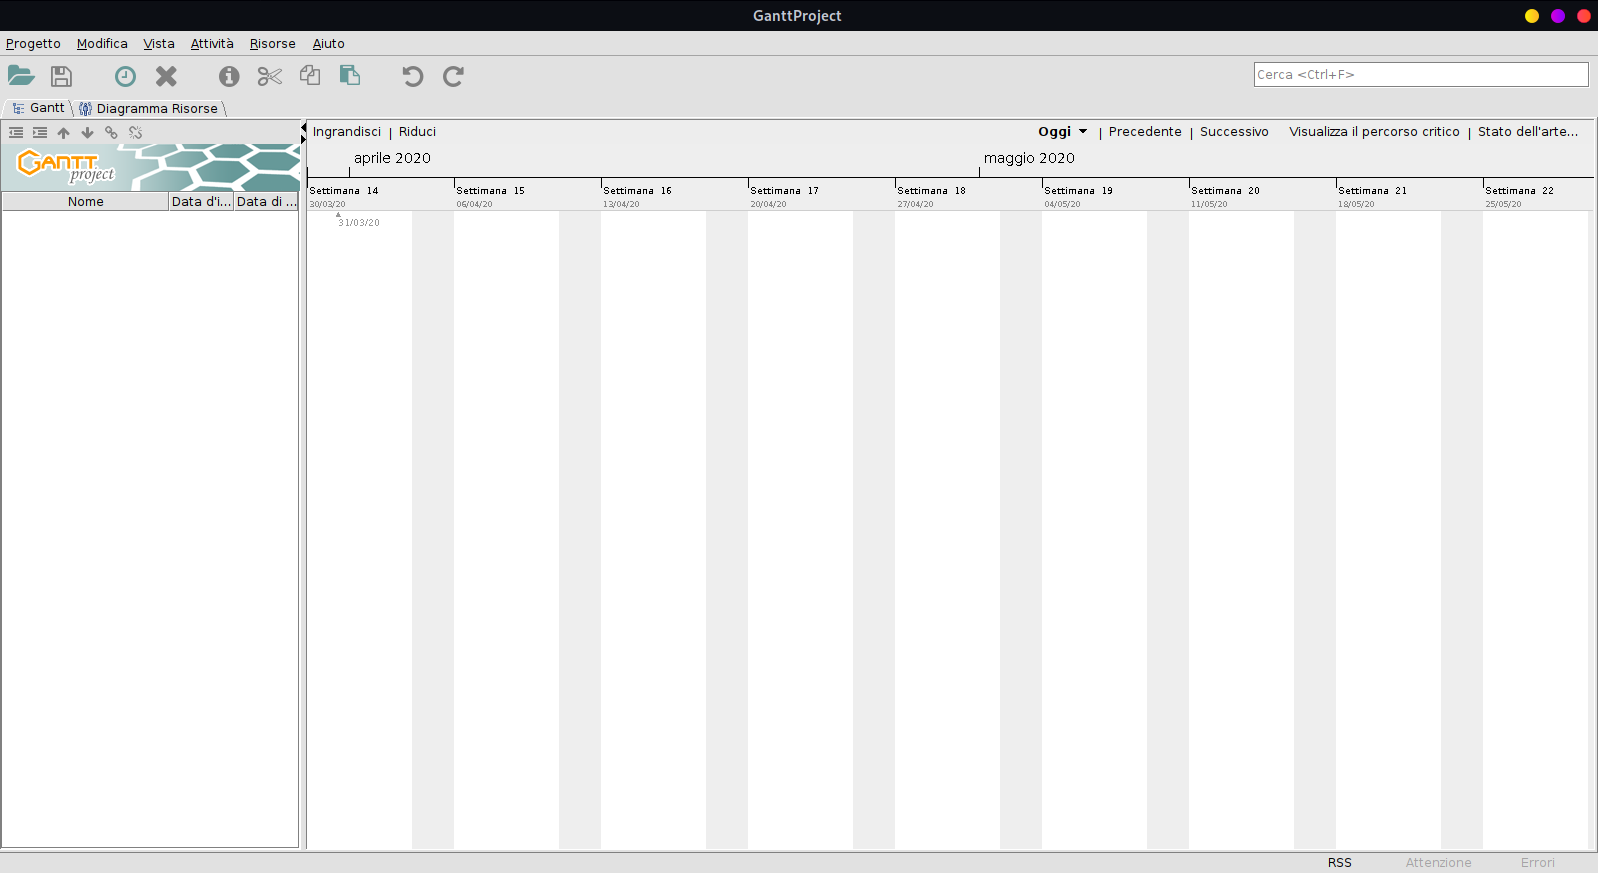
\includegraphics[width=15cm]{img/gantt.png}
  \label{fig:gantt}
  \caption{GanttProject per GNU/Linux.}
\end{figure}

\paragraph{Google Sheets}
Google Sheets è un programma, appartenente alla \glossario{suite} office di Google, per la creazione di fogli di calcolo. Questo applicativo viene usato dal gruppo per la creazione delle tabelle e dei grafici presenti nel \textsc{Piano di Progetto}, e per lo svolgimento dei calcoli dei preventivi presenti nello stesso documento.

\begin{figure}[H]
  \centering
  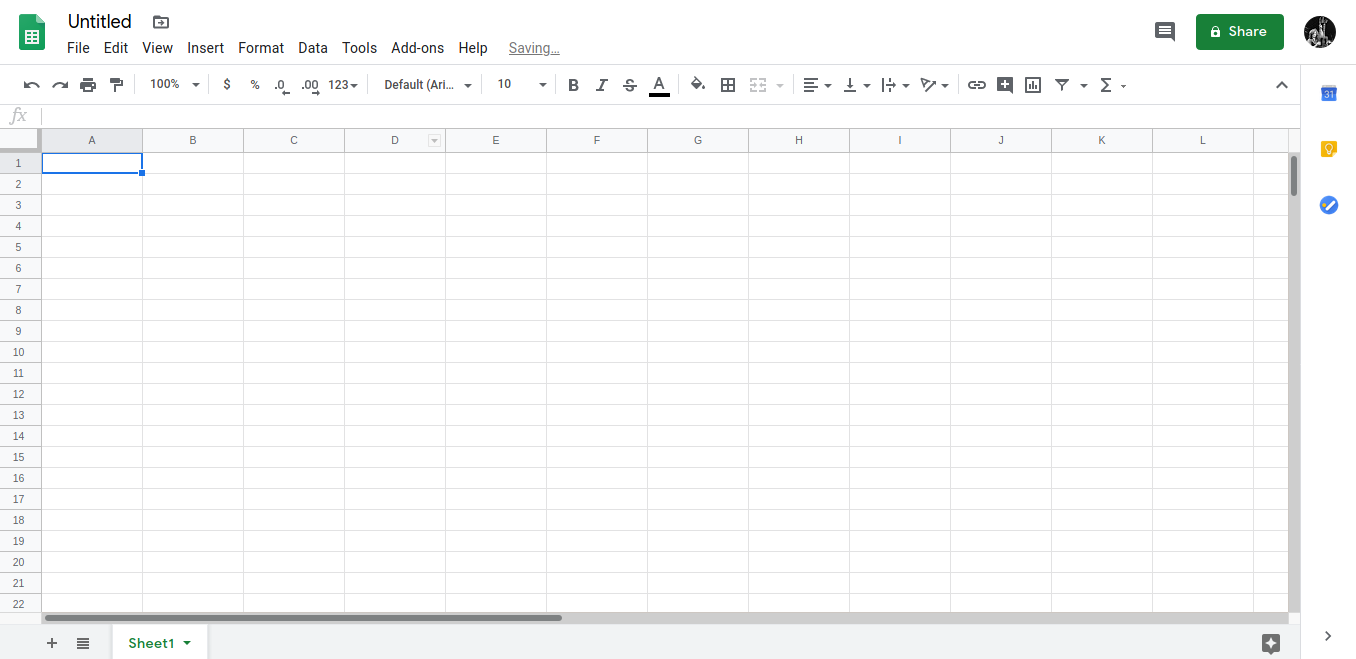
\includegraphics[width=15cm]{img/sheets.png}
  \label{fig:sheets}
  \caption{Piattaforma online \href{https://docs.google.com/spreadsheets/u/0/}{Google Sheets}.}
\end{figure}
%%% EVENTUALI ALTRI STRUMENTI

%%%%%%%%%%%%%%%%%%%%%%%
%%% 2.2 - SVILUPPO %%%
%%%%%%%%%%%%%%%%%%%%%%%
\subsection{Sviluppo}

\subsubsection{Scopo}
Lo scopo del processo di sviluppo è descrivere le attività che il gruppo deve svolgere al fine di realizzare il prodotto finale richiesto dal proponente.

\subsubsection{Aspettative}
Le aspettative di questo processo sono le seguenti:
\begin{itemize}
  \item Stabilire gli obiettivi di sviluppo;
  \item Stabilire i vincoli tecnologici e di design;
  \item Realizzare un prodotto finale che soddisfi i requisiti richiesti dal proponente e superi correttamente i test.
\end{itemize}

\subsubsection{Descrizione}
Il processo di sviluppo si articola nelle seguenti attività:
\begin{itemize}
  \item Analisi dei Requisiti;
  \item Progettazione;
  \item Codifica.
\end{itemize}

\subsubsection{Attività}
\paragraph{Analisi dei requisiti}
\subparagraph{Scopo}
Lo scopo dell'\textsc{Analisi dei Requisiti}, redatta dagli analisti, definisce e quindi elenca tutti i requisiti del capitolato. Questi vengono estrapolati da diverse fonti:
\begin{itemize}
  \item Capitolato d'appalto e relativo approfondimento;
  \item Riunioni esterne con il proponente;
  \item Casi d'uso.
\end{itemize}
Il documento corrispondente conterrà quindi:
\begin{itemize}
  \item La descrizione generale del prodotto;
  \item I casi d'uso;
  \item Il tracciamento dei requisiti individuati a partire dalle richieste del cliente e dai casi d'uso.
\end{itemize}

\subparagraph{Aspettative}
L'aspettativa di questo processo coincide con la creazione del documento \textsc{Analisi dei Requisiti}, il quale contiene appunto i requisiti richiesti dal proponente per la realizzazione del progetto.

\subparagraph{Classificazione dei casi d'uso}
I casi d'uso vengono classificati e identificati secondo uno schema univoco, al fine di facilitarne la lettura e la comprensione. La classificazione segue la seguente codifica: \\
\begin{center}
  \centering
  \textbf{UC[P].[F].[FF].[FFF]}
\end{center} dove:
\begin{itemize}
  \item \textbf{UC}: indica che il codice è un caso d'uso;
  \item \textbf{P}: consistente in un numero progressivo, identifica il caso;
  \item \textbf{F}, \textbf{FF} e \textbf{FFF}: consistenti ognuno di un numero progressivo, identificano il sottocaso.
\end{itemize}
Ogni caso d'uso è formato, non necessariamente integralmente, dai seguenti campi:
\begin{itemize}
  \item \textbf{\glossario{Diagrammi UML}}: diagrammi esplicativi realizzati in linguaggio UML2.0;
  \item \textbf{Attori primari}: attori primari del caso d'uso;
  \item \textbf{Attori secondari}: attori secondari del caso d'uso;
  \item \textbf{Descrizione}: descrizione del caso d'uso;
  \item \textbf{Precondizione}: condizioni che devono essere soddisfatte perché gli eventi del caso d'uso si possano verificare;
  \item \textbf{Scenario principale}: flusso degli eventi del caso d'uso;
  \item \textbf{Postcondizione}: condizioni che devono essere soddisfatte dopo il verificarsi degli eventi;
  \item \textbf{Estensioni}: estensioni coinvolte;
  \item \textbf{Generalizzazioni}: generalizzazioni coinvolte.
\end{itemize}

\subparagraph{Classificazione dei requisiti}
Anche i requisiti sono identificati secondo uno schema univoco; questo è così composto: \\
\begin{center}
  \centering
  \textbf{R[T]-[P]-[I]}
\end{center} dove:
\begin{itemize}
  \item \textbf{R}: indica che il codice è un requisito;
  \item \textbf{T}: indica la tipologia del requisito. Il requisito può essere:
  \begin{itemize}
    \item \textbf{F}: funzionale;
    \item \textbf{P}: prestazionale;
    \item \textbf{Q}: qualitativo;
    \item \textbf{V}: vincolo.
  \end{itemize}
  \item \textbf{P}: indica la priorità del requisito. Questa può essere:
  \begin{itemize}
    \item \textbf{O}: indica un requisito obbligatorio poiché necessario;
    \item \textbf{D}: indica un requisito desiderabile, ma non necessario;
    \item \textbf{F}: indica un requisito opzionale o contrattabile in corso d'opera del progetto.
  \end{itemize}
  \item \textbf{I}: indica l'identificativo del requisito nella forma \\
  \begin{center}
    \centering
    \textbf{codicePadre.codiceFiglio}
  \end{center} dove entrambi i codici sono numeri progressivi.
\end{itemize}


\paragraph{Progettazione}
\subparagraph{Scopo}
L'attività di progettazione si colloca temporalmente tra l'analisi dei requisiti e la codifica; durante questa attività i progettisti definiscono una soluzione al problema di partenza per soddisfare i requisiti definiti. \\
Lo scopo della progettazione è quindi comprendere le caratteristiche del prodotto richiesto e definire l'architettura logica di quanto si deve sviluppare, garantendo l'efficacia del prodotto e l'efficienza nella realizzazione di questo.

\subparagraph{Aspettative}
L'aspettativa di questa attività coincide con la realizzazione dell'architettura logica del sistema, la quale dovrà perseguire i seguenti obiettivi di qualità:
\begin{itemize}
  \item \textbf{Sufficienza}: la capacità di soddisfare tutti i requisiti rilevati;
  \item \textbf{Comprensibilità}: deve essere comprensibile da tutti gli \glossario{stakeholder};
  \item \textbf{Modularità}: deve essere suddivisibile in parti chiare e distinte, il più possibile non sovrapponibili tra loro;
  \item \textbf{Robustezza}: deve essere in grado di gestire input diversi da parte dell'utente;
  \item \textbf{Flessibilità}: deve essere modificabile al variare dei requisiti con un costo contenuto;
  \item \textbf{Efficienza}: deve gestire le risorse minimizzando gli sprechi di queste;
  \item \textbf{Affidabilità}: deve eseguire quello per cui è progettata nella maniera corretta;
  \item \textbf{Disponibilità}: il sistema non deve influire eccessivamente sull'utenza quando si trova in manutenzione e, quindi, non disponibile;
  \item \textbf{Sicurezza}: non deve essere vulnerabile alle intrusioni e non deve presentare gravi malfunzionamenti;
  \item \textbf{Semplicità}: deve soddisfare i requisiti necessari senza possedere funzionalità superflue;
  \item \textbf{Incapsulamento}: deve nascondere correttamente la struttura interna rendendola quanto più possibile indipendente dall'esterno, in modo da rendere invisibili eventuali modifiche;
  \item \textbf{Coesione}: deve essere composta da componenti raggruppate per funzionalità e il meno possibile interdipendenti tra loro;
  \item \textbf{Basso accoppiamento}: deve essere composta da parti distinte, il meno possibile dipendenti l'una dall'altra.
\end{itemize}

\subparagraph{Descrizione}
Questa attività si divide nelle seguenti parti:
\begin{itemize}
  \item \textbf{Progettazione architetturale}: definizione ad alto livello dell'architettura e delle componenti del sistema;
  \item \textbf{Progettazione di dettaglio}: definizione nel dettaglio delle singole componenti del sistema e delle interazioni che sussistono tra di esse. Sono qui definiti anche i diagrammi che descrivono l'architettura e le componenti del sistema.
\end{itemize}

Sono definite due \glossario{milestone}:
\begin{itemize}
  \item La \textbf{\glossario{Technology Baseline}};
  \item La \textbf{\glossario{Product Baseline}}.
\end{itemize}

\subparagraph*{Technology Baseline}
La Technology Baseline ha come scopo:
\begin{itemize}
  \item La motivazione delle scelte del gruppo per quanto concerne l'uso di determinate tecnologie, \glossario{framework} e \glossario{librerie};
  \item La presentazione di un \glossario{Proof of Concept}, ossia un eseguibile parziale del sistema con funzione dimostrativa sviluppato con le tecnologie scelte. Il proof of concept funge anche da \glossario{baseline} per il successivo sviluppo.
\end{itemize}

\subparagraph*{Product Baseline}
Nella Product Baseline vengono presentati:
\begin{itemize}
  \item La \glossario{baseline} architetturale del prodotto;
  \item La descrizione dei \glossario{design pattern} utilizzati nella definizione dell'architettura;
  \item I diagrammi UML, che rendono più chiare le soluzioni progettuali adottate;
  \item I test di unità.
\end{itemize}
I diagrammi UML e i design pattern saranno inclusi in un \textsc{Allegato Tecnico} opportunamente redatto e consegnato.\\
I diagrammi UML consistono in diagrammi utilizzati per rendere più chiare le scelte progettuali; questi sono divisi in:
\begin{itemize}
  \item \textbf{Diagrammi delle classi}: rappresentano gli oggetti del sistema e le relazioni che sussistono tra essi;
  \item \textbf{Diagrammi dei package}: rappresentano le dipendenze tra classi raggruppate in package;
  \item \textbf{Diagrammi di attività}: descrivono un processo;
  \item \textbf{Diagrammi di sequenza}: descrivono una sequenza di processi.
\end{itemize}

% per eventuali approfondimenti del gruppo sui diagrammi: leggere le slide del professore %

\subparagraph*{Diagrammi delle classi}
I diagrammi delle classi rappresentano i tipi di oggetti che fanno parte del sistema e le relazioni tra questi. Le classi dovranno presentare le seguenti caratteristiche:
\begin{itemize}
  \item \textbf{Nome}: nome della classe;
  \item \textbf{Attributi}: campo opzionale, rappresentano i membri della classe; posseggono le seguenti proprietà:
    \begin{itemize}
      \item \textbf{Visibilità}: visibilità dell'attributo rispetto alle altre classi. Essa può essere:
      \begin{itemize}
        \item Public;
        \item Protected;
        \item Package;
        \item Private.
      \end{itemize}
      \item \textbf{Nome dell'attributo};
      \item \textbf{Tipo di dato};
      \item \textbf{Molteplicità}: campo opzionale indicante il numero di occorrenze dell'attributo nella classe;
      \item \textbf{Default}: campo opzionale indicante il valore di default dell'attributo;
      \item \textbf{Proprietà aggiuntive}: campo opzionale.
    \end{itemize}
    \item \textbf{Operazioni}: campo opzionale, rappresentano le operazioni che la classe può eseguire; posseggono le seguenti proprietà:
    \begin{itemize}
      \item \textbf{Visibilità}: visibilità dell'operazione rispetto alle altre classi. Valgono le stesse opzioni enunciate per la visiblità degli attributi;
      \item \textbf{Nome dell'operazione};
      \item \textbf{Parametri}: campo opzionale, contiene:
      \begin{itemize}
        \item La lista dei parametri;
        \item La direzione, che può essere \textit{in}, \textit{out}, \textit{in-out}.
      \end{itemize}
      \item \textbf{Tipo di ritorno};
      \item \textbf{Proprietà aggiuntive}: campo opzionale.
    \end{itemize}
  \item \textbf{Relazioni}: campo opzionale, rappresentano il tipo di relazione che sussiste tra due classi; esse possono essere:
  \begin{itemize}
    \item \textbf{Dipendenza}: quando un metodo della classe rivece come parametro un'istanza di un'altra classe o quando la classe utilizza un'oggetto di un'altra classe;
    \item \textbf{Aggregazione}: quando la classe possiede un riferimento a un oggetto condiviso da un'altra classe;
    \item \textbf{Composizione}: quando la classe contiene oggetti di un'altra classe;
    \item \textbf{Associazione}: quando la classe crea e usa un oggetto di un'altra classe;
    \item \textbf{Generalizzazione}: quando la classe è un'istanza che specializza un'altra classe.
  \end{itemize}
\end{itemize}

\subparagraph*{Diagrammi dei package}
Un package è un raggruppamento di un numero arbitrario di elementi UML in un'unità di livello più alto. I diagrammi dei package documentano le dipendenze fra le classi, e ciò consente l'individuazione di dipendenze tra le classi. In particolar modo, essi permettono di individuare eventuali dipendenze circolari tra classi, permettendo la loro rimozione.

\subparagraph*{Diagrammi di attività}
I diagrammi di attività descrivono la logica procedurale dei processi che compongono il software. Essi aiutano a descrivere gli aspetti dinamici dei casi d'uso, mostrando le attività che possono accadere e le sequenze di azioni con cui vengono svolte. \\
Questi diagrammi sono composti da:
\begin{itemize}
  \item \textbf{Nodo iniziale}: da dove inizia l'esecuzione del processo;
  \item \textbf{Nodo finale}: dove finisce il processo;
  \item \textbf{Fork}: punto di divisione per l'elaborazione parallela;
  \item \textbf{Join}: sincronizzazione tra due o più flussi di elaborazione parallela, generati da un fork;
  \item \textbf{Branch}: rami decisionali in cui si può intraprendere solo uno dei percorsi.
\end{itemize}

\subparagraph*{Diagrammi di sequenza}
I diagrammi di sequenza descrivono delle sequenze di azioni in cui tutte le scelte sono già state effettuate; in esso non compaiono quindi scelte o flussi alternativi. \\
I diagrammi di sequenza si presentano come una serie di oggetti che si scambiano messaggi, collocati in linee parallele che indicano l'avanzare del tempo; essi sono costituiti da:
\begin{itemize}
  \item \textbf{Partecipanti}: entità che detengono il flusso del caso d'uso. I partecipanti sono composti da:
  \begin{itemize}
    \item \textbf{Nome};
    \item \textbf{Barra di attivazione}: opzionale, indica in quale momento un partecipante è attivo.
  \end{itemize}
  \item \textbf{Messaggi}: dati e operazioni scambiati tra i partecipanti. Un messaggio può essere:
  \begin{itemize}
    \item \textbf{Sincrono}: chiamata in cui il partecipante chiamante aspetta la risposta del partecipante chiamato prima di continuare l'esecuzione;
    \item \textbf{Asincrono}: chiamata in cui il partecipante chiamante non aspetta la risposta del partecipante chiamato, ma continua l'esecuzione subito dopo la chiamata;
    \item \textbf{Di ritorno}: messaggio di ritorno dopo un messaggio di chiamata;
    \item \textbf{Di creazione}: messaggio di creazione di un nuovo partecipante;
    \item \textbf{Di distruzione}: messaggio di distruzione di un partecipante.
  \end{itemize}
  \item \textbf{Frame di interazione}: un ciclo o una condizione che contiene una porzione di diagramma. Esso è composto da:
  \begin{itemize}
    \item \textbf{Guardia}: condizione di attivazione del frame;
    \item \textbf{Etichetta}: tipologia del frame; questo infatti può essere:
    % minuscole perché sono termini propri, non è un errore
    \begin{itemize}
      \item \textbf{alt}: alternativa tra frammenti multipli, viene eseguito solo quello per cui è verificata la condizione;
      \item \textbf{opt}: opzionale, il frammento viene eseguito solo se la condizione specificata è verificata;
      \item \textbf{par}: parallelo, ossia ogni frammento viene eseguito in parallelo;
      \item \textbf{loop}: ciclo, il frammento può essere eseguito più volte in base alla guardia;
      \item \textbf{region}: regione critica, il frammento può essere eseguito da un solo \glossario{thread} alla volta;
      \item \textbf{neg}: negativo, il frammento mostra un'interazione non valida;
      \item \textbf{ref}: riferimento, si riferisce a un'interazione definita in un altro diagramma;
      \item \textbf{sd}: sequence diagram, usato come contenitore di un intero diagramma di sequenza.
    \end{itemize}
  \end{itemize}
\end{itemize}

\paragraph{Codifica}
\subparagraph{Scopo}
Lo scopo di questa attività è quella di fornire le regole per la scrittura del codice JavaScript. La codifica coincide con la programmazione stessa del prodotto; è quindi a opera dei \glossario{Programmatori}, i quali dovranno seguire le seguenti regole al fine di ottenere un prodotto coerente e uniforme in tutte le sue componenti. \\
Tale sezione potrà poi venire ampliata nel caso in cui il gruppo senta l'esigenza di ulteriori norme in tale senso, o si renda necessario l'utilizzo di altri linguaggi di programmazione in aggiunta a JavaScript.
\subparagraph{Aspettative}
Le aspettative di questo processo sono:
\begin{itemize}
  \item Ottenere un prodotto software conforme ai requisiti concordati con il proponente;
  \item Assicurare l'uniformità di produzione delle diverse componenti del prodotto;
  \item Assicurare che il codice prodotto sia:
  \begin{itemize}
    \item Uniforme nella sua struttura;
    \item Leggibile e di facile comprensione, nell'ottica della futura verifica, validazione e manutenzione del prodotto.
  \end{itemize}
\end{itemize}
\subparagraph{Descrizione}
Il codice dovrà essere scritto rispettando quanto documentato; nello specifico, esso dovrà perseguire gli obiettivi di qualità definiti nel documento \textsc{Piano di Qualifica v2.0.0}.

\subparagraph{Versione del linguaggio}
Il codice JavaScript dovrà essere scritto seguendo la specifica tecnica \glossario{ECMAScript 6}, conosciuto anche come ES6 o ES-2015.

\subparagraph{Intestazione}
Ogni file contenente codice deve possedere la seguente intestazione:
\begin{lstlisting}
 /*
 * File: nome file
 * Version: versione file
 * Date: data creazione
 * Author: nome autore
 * Description: breve descrizione file
 * Remarks: eventuali appunti da fare (avvertenze, dipendenze)
 */
\end{lstlisting}
In aggiunta a questo, è possibile utilizzare la \glossario{keyword} TODO per indicare codice temporaneo e soluzioni migliorabili in un secondo momento.

\subparagraph{Stile}
Al fine di ottenere una scrittura omogenea e uniforme del codice, ogni membro del gruppo è tenuto a rispettare le norme che seguono.

\subparagraph*{Variabili e funzioni}
Le funzioni e le variabili locali seguono la codifica \glossario{camelCase}:
\begin{itemize}
  \item Iniziano con una lettera minuscola;
  \item In caso di variabili composte da più parole, ogni parola deve cominciare con la lettera maiuscola, ad eccezione della prima.
\end{itemize}
Le variabili globali dovranno invece essere scritte in stampatello maiuscolo. \\
In aggiunta a questo, ogni variabile e funzione deve avere un nome significativo, al fine di essere facilmente riconducibile al suo scopo. \\
Le variabili locali, infine, devono essere sempre dichiarate con l'utilizzo della keyword \textbf{let}.

\subparagraph*{Indentazione}
I blocchi, ad eccezione dei commenti, devono seguire la corretta indentazione, consistente di due spazi per ciascun livello d'indentazione. È vietato l'uso di tabulazioni, poiché consistenti di caratteri diversi in diversi sistemi operativi; l'\glossario{IDE} di ciascun membro del gruppo deve quindi essere configurato perché la tabulazione corrisponda a due spazi.

\subparagraph*{Spazi e capo riga}
Non è richiesto l'utilizzo di spazi precedenti e conseguenti agli operatori; è tuttavia buona pratica farne utilizzo in caso di \textit{statements} complessi. \\
Tutti i capo riga dovranno essere LF (line feed); l'utilizzo di CRLF non è ammesso, poiché non riconosciuto da sistemi operativi diversi da Microsoft Windows.

\subparagraph*{Punto e virgola}
Ogni \textit{statement} deve finire con il carattere punto e virgola \textbf{;}. Sebbene l'utilizzo di questi sia opzionale in linguaggio JavaScript, questa regola permette una comprensione più chiara degli \textit{statements}.

\subparagraph*{Impostazione dei blocchi}
I blocchi di codice devono seguire le seguenti regole:
\begin{itemize}
  \item \textbf{Righe vuote}: deve essere sempre presente una riga vuota prima e dopo ogni blocco;
  \item \textbf{Parentesi}: i blocchi di codice consistenti di più di una riga devono essere racchiusi tra parentesi graffe, le quali devono cominciare nella stessa riga del codice. I blocchi di codice consistenti di un'unica riga possono essere scritti senza parentesi. \\ Nel caso degli \textit{statements} \textbf{if-else-if} e dei cicli iterativi, le keyword \textbf{else} ed \textbf{else if} devono essere inserite nella stessa riga della parentesi graffa che chiude il blocco \textbf{if}.
\end{itemize}

\subsubsection{Strumenti}
Durante il processo di sviluppo verranno utilizzati diversi strumenti software.

\paragraph{Visual Studio Code}
Visual Studio Code è l'IDE che viene uniformemente usato da ogni componente del gruppo. Questo strumento software permette l'estensione delle funzionalità attraverso l'installazione di componenti aggiuntivi. \\
Esso viene utilizzato sia per lo redazione dei documenti che per la scrittura del codice

\begin{figure}[H]
  \centering
  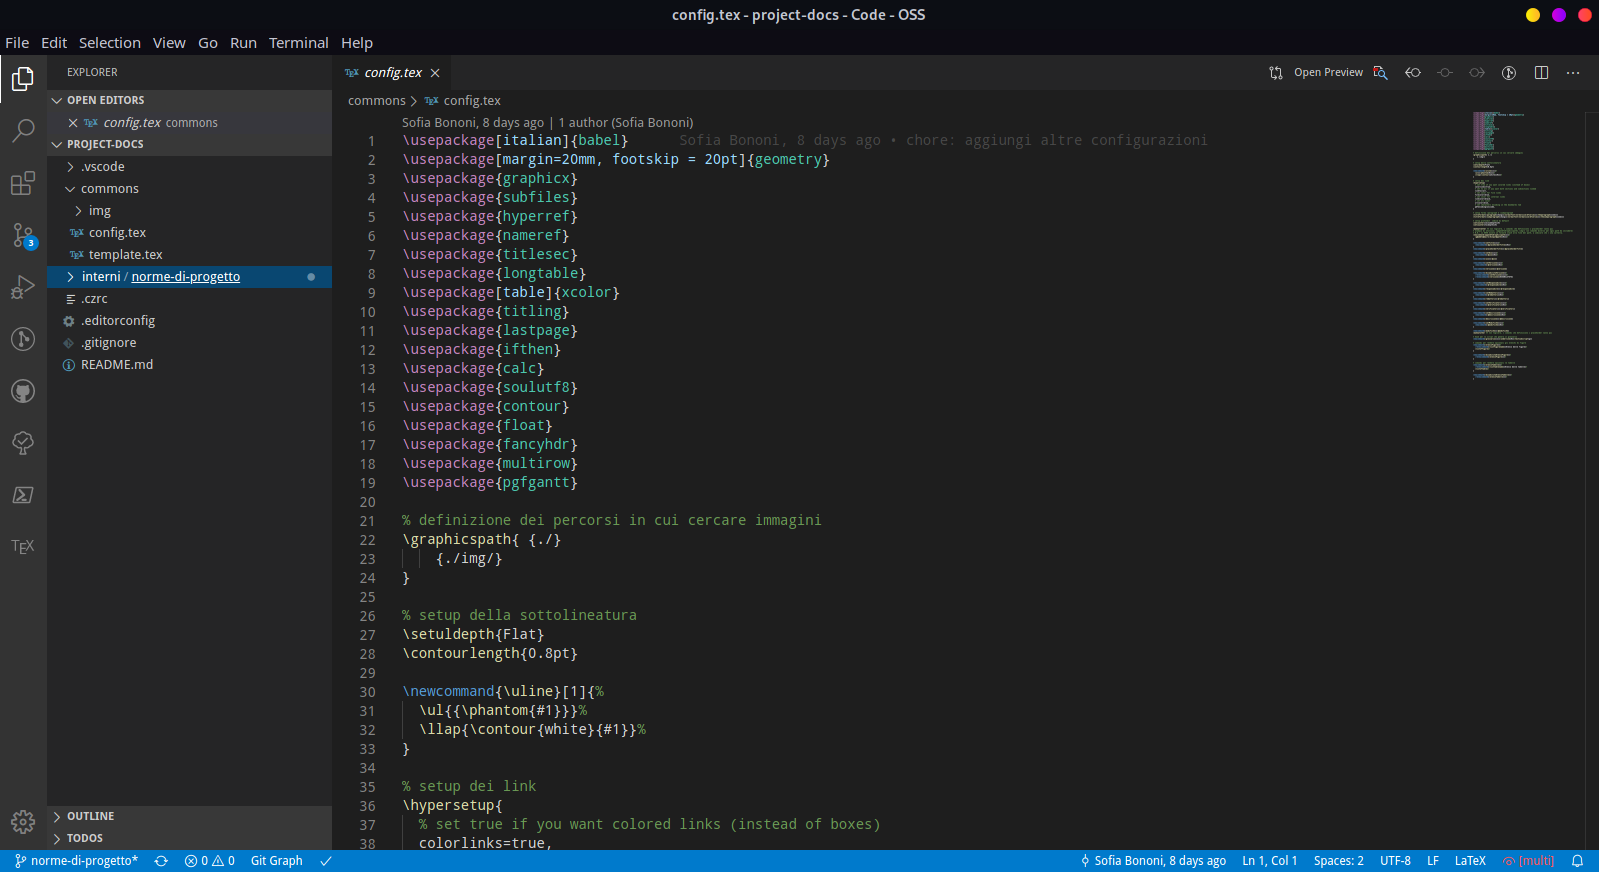
\includegraphics[width=15cm]{img/vscode.png}
  \label{fig:github}
  \caption{Visual Studio Code per GNU/Linux.}
\end{figure}

\paragraph{ESLint}
\glossario{ESLint} è uno strumento di analisi statica del codice che identifica all'interno di questo eventuali problemi o discordanze da quanto definito nella normazione dell'attività di codifica.

\paragraph{PlantUML}
Viene utilizzato lo strumento PlantUML per lo sviluppo dei grafici UML dei casi d'uso presenti nell'\textsc{Analisi dei Requisiti v2.0.0}.

\paragraph{Yarn}
\glossario{Yarn} è un gestore di pacchetti per il linguaggio di programmazione JavaScript. Esso viene utilizzato dal gruppo per l'installazione dei pacchetti necessari allo sviluppo e all'esecuzione del codice.

\paragraph{Grafana}
Grafana è un software open-source per l'analisi dati e l'interazione con questi. Questo strumento viene utilizzato dal gruppo come sistema sul quale sviluppare il plug-in richiesto dall'azienda proponente.

\paragraph{Docker}
Docker è un software che permette la creazione di \glossario{container} GNU/Linux. Questo strumento verrà utilizzato dal gruppo per la configurazione dell'ambiente di Grafana e, quindi, lo sviluppo del plug-in richiesto dal capitolato.

\paragraph{Estensioni del linguaggio}
\subparagraph{Node.js}
\glossario{Node.js} è una \glossario{runtime} open-source per l'esecuzione di codice JavaScript, costruita sul motore \glossario{JavaScript V8} di \glossario{Google Chrome}. Essa viene usata del gruppo per lo sviluppo del programma di addestramento e del plug-in, richiesti dal proponente.

\subparagraph{Electron}
Electron è un framework open-source che combina il \glossario{motore di rendering} \glossario{Chromium} e la runtime Node.js, che permette lo sviluppo della \glossario{GUI} di applicazioni desktop utilizzando tecnologie web. Esso viene usato dal gruppo per lo sviluppo del programma di addestramento.

\subparagraph{React}
\glossario{React} è una libreria Javascript per lo sviluppo di applicazioni web e interfacce utente. Esso viene usato per lo sviluppo del plug-in di Grafana richiesto dal capitolato.

\newpage

\end{document}
